\chapter{Arhitektura i dizajn sustava}

\section{Baza podataka}

\paragraph{}
{Za potrebe razvoja aplikacije SpotPicker koristi se relacijska baza podataka. 
Osnovne zadaće baze podataka su pohrana i organizacija podataka te brzo pretraživanje 
i dohvaćanje podataka kako bi ih se moglo dalje obraditi.
Svaki je entitet korištene relacijske baze naveden i opisan u daljnjem tekstu, 
a ispod opisa nalazi se tablični prikaz opisanog entiteta i njegovih atributa.}

\paragraph{}{Baza podataka aplikacije SpotPicker sastoji se od sljedećih entiteta:}
\begin{packed_item}
	\item ConfirmationLink
	\item Korisnik
	\item Parking
	\item Rezervacija
	\item Wallet
\end{packed_item}


\subsection{Opis tablica}

\paragraph{}
{\emph{ConfirmationLink}\\
Entitet ConfirmationLink sadrži informacije vezane za potvrđene korisnike i sadrži sljedeće atribute:
ConformationLinkID, KorisnikID, Link i isValid. Primarni ključ entiteta ConfirmationLink je atribut ConformationLinkID, a strani ključ je atribut KorisnikID.
Navedeni je entitet u vezi \emph{One-to-One} s entitetom Korisnik preko atributa KorisnikID.}

	\begin{longtblr}[
					label=none,
					entry=none
					]{
						width = \textwidth,
						colspec={|X[6,l]|X[6, l]|X[20, l]|}, 
						rowhead = 1,
					} %definicija širine tablice, širine stupaca, poravnanje i broja redaka naslova tablice
					\hline \SetCell[c=3]{c}{\textbf{ConfirmationLink}}	 \\ \hline[3pt]
					\SetCell{LightGreen}Confirmation LinkID & INT	&  	TO DO  	\\ \hline
					\SetCell{LightBlue} Korisnik ID	& INT & jedinstveni ID korisnika 	\\ \hline
					Link	& NVARCHAR &  TO DO	\\ \hline 
					isValid & BIT &  informacija o potvrdi korisnika \\ \hline  
	\end{longtblr} \\

\paragraph{}
{\emph{Korisnik}\\
Entitet Korisnik sadrži informacije vezane za registrirane korisnike aplikacije i sadrži sljedeće atribute:
KorisnikID, Username, Password, RazinaPristupa, Name, Surname, PictureData, BankAccountNumber, Email, AccountEnabled i EmailVerified. 
Primarni ključ entiteta Korisnik je KorisnikID. 
Navedeni je entitet u vezi \emph{One-to-Many} s entitetom ConfirmationLink preko atributa KorisnikID, 
vezi \emph{One-to-Many} s entitetom Parking preko atributa KorisnikID, 
u vezi \emph{One-to-Many} s entitetom Rezervacija preko atributa KorisnikID 
i u vezi \emph{One-to-One} s entitetom Wallet preko atributa KorisnikID.}

	\begin{longtblr}[
					label=none,
					entry=none
					]{
						width = \textwidth,
						colspec={|X[6,l]|X[6, l]|X[20, l]|}, 
						rowhead = 1,
					} %definicija širine tablice, širine stupaca, poravnanje i broja redaka naslova tablice
					\hline \SetCell[c=3]{c}{\textbf{Korisnik}}	 \\ \hline[3pt]
					\SetCell{LightGreen}KorisnikID & INT	&  	jedinstveni ID korisnika  	\\ \hline
					Username	& NVARCHAR &  korisničko ime	\\ \hline 
					Password & NVARCHAR &  TO DO \\ \hline 
					Razina Pristupa & INT & TO DO	\\ \hline 
					Name	& VARCHAR &   ime korisnika	\\ \hline
					Surname	& VARCHAR &  prezime korisnika \\ \hline
					PictureData	& VARBINARY &   TO DO	\\ \hline
					BankAccount Number	& VARCHAR &  broj bankovnog računa korisnika	\\ \hline
					Email	& VARCHAR &   korisnikova e-mail adresa	\\ \hline
					Account Enabled	& BIT &  informacija o potvrdi profila korisnika od strane administratora	\\ \hline
					Email Verified	& BIT &   informacija o potvrdi profila korisnika putem e-maila	\\ \hline
	\end{longtblr} \\

\paragraph{}
{\emph{Parking}\\
Entitet Parking sadrži informacije vezane za opis i konfiguraciju parkirališta te sadrži sljedeće atribute:
ParkingID koji je primarni ključ entiteta, Name, Description, Photo, PricePerHour, Capacity i KorisnikID. Strani ključ entiteta \emph{Parking} je KorisnikID.
Navedeni je entitet u vezi \emph{Many-to-One} s entitetom Korisnik preko atributa KorisnikID, 
i u vezi \emph{One-to-Many} s entitetom Rezervacija preko atributa ParkingID.
}

	\begin{longtblr}[
					label=none,
					entry=none
					]{
						width = \textwidth,
						colspec={|X[6,l]|X[6, l]|X[20, l]|}, 
						rowhead = 1,
					} %definicija širine tablice, širine stupaca, poravnanje i broja redaka naslova tablice
					\hline \SetCell[c=3]{c}{\textbf{Parking}}	 \\ \hline[3pt]
					\SetCell{LightGreen}ParkingID & INT	&  	jedinstveni ID parkirališta  	\\ \hline
					Name	& NVARCHAR &  naziv parkirališta	\\ \hline 
					Description & VARCHAR &  opis parkirališta \\ \hline 
					Photo & VARBINARY	&  	TO DO	\\ \hline 
					PricePerHour & INT	&  	cijena parkirališnog mjesta po satu	\\ \hline
					Capacity & INT	&  	broj parkirališnih mjesta na parkiralištu	\\ \hline
					\SetCell{LightBlue} KorisnikID	& INT &  jedinstveni ID korisnika	\\ \hline 
	\end{longtblr} \\
	
\paragraph{}
{\emph{Rezervacija}\\
Entitet Rezervacija sadrži informacije vezanie za rezervacije pojedinih parkirnih mjesta i sadrži sljedeće atribute:
ReservationID koji je primarni ključ entiteta, KorisnikID, ParkingID, DateTimeStart, DateTimeEnd i ParkingPlaceId. Strani ključevi entiteta \emph{Rezervacija} su KorisnikID i ParkingID.
Navedeni je entitet u vezi \emph{Many-to-One} s entitetom Korisnik preko atributa KorisnikID.
}

	\begin{longtblr}[
					label=none,
					entry=none
					]{
						width = \textwidth,
						colspec={|X[6,l]|X[6, l]|X[20, l]|}, 
						rowhead = 1,
					} %definicija širine tablice, širine stupaca, poravnanje i broja redaka naslova tablice
					\hline \SetCell[c=3]{c}{\textbf{Rezervacija}}	 \\ \hline[3pt]
					\SetCell{LightGreen} ReservationID & INT	&  	jedinstveni ID rezervacije  	\\ \hline
					\SetCell{LightBlue} KorisnikID	& INT &   jedinstveni ID korisnika	\\ \hline 
					\SetCell{LightBlue} ParkingID	& INT &  jedinstveni ID parkirališta 	\\ \hline 
					DateTimeStart	& DATETIME &  početno datum-vrijeme rezervacije  	\\ \hline 
					DateTimeEnd & DATETIME &  završno datum-vrijeme rezervacije \\ \hline 
					ParkingPlace ID & INT	&  	jedinstveni ID parkirališnog mjesta	\\ \hline 
	\end{longtblr} \\
	
\paragraph{}
{\emph{Wallet}\\
Entitet Wallet sadrži informacije vezane za novčanik korisnika i njegova sredstva. Sadrži sljedeće atribute:
WalletID koji je primarni ključ entiteta, KorisnikID koji je strani ključ entiteta i Balance.
Navedeni je entitet u vezi \emph{One-to-One} s entitetom Korisnik preko atributa KorisnikID.
}

	\begin{longtblr}[
					label=none,
					entry=none
					]{
						width = \textwidth,
						colspec={|X[6,l]|X[6, l]|X[20, l]|}, 
						rowhead = 1,
					} %definicija širine tablice, širine stupaca, poravnanje i broja redaka naslova tablice
					\hline \SetCell[c=3]{c}{\textbf{Wallet}}	 \\ \hline[3pt]
					\SetCell{LightGreen}WalletID & INT	&  	jedinstveni ID novčanika  	\\ \hline
					\SetCell{LightBlue} KorisnikID	& VARCHAR &   jedinstveni ID korisnika	\\ \hline 
					Balance	& MONEY &   iznos sredstava u novčaniku korisnika	\\ \hline 
	\end{longtblr}\\
	


\subsection{Dijagram baze podataka}

\begin{figure}[!htb]
	\centering
	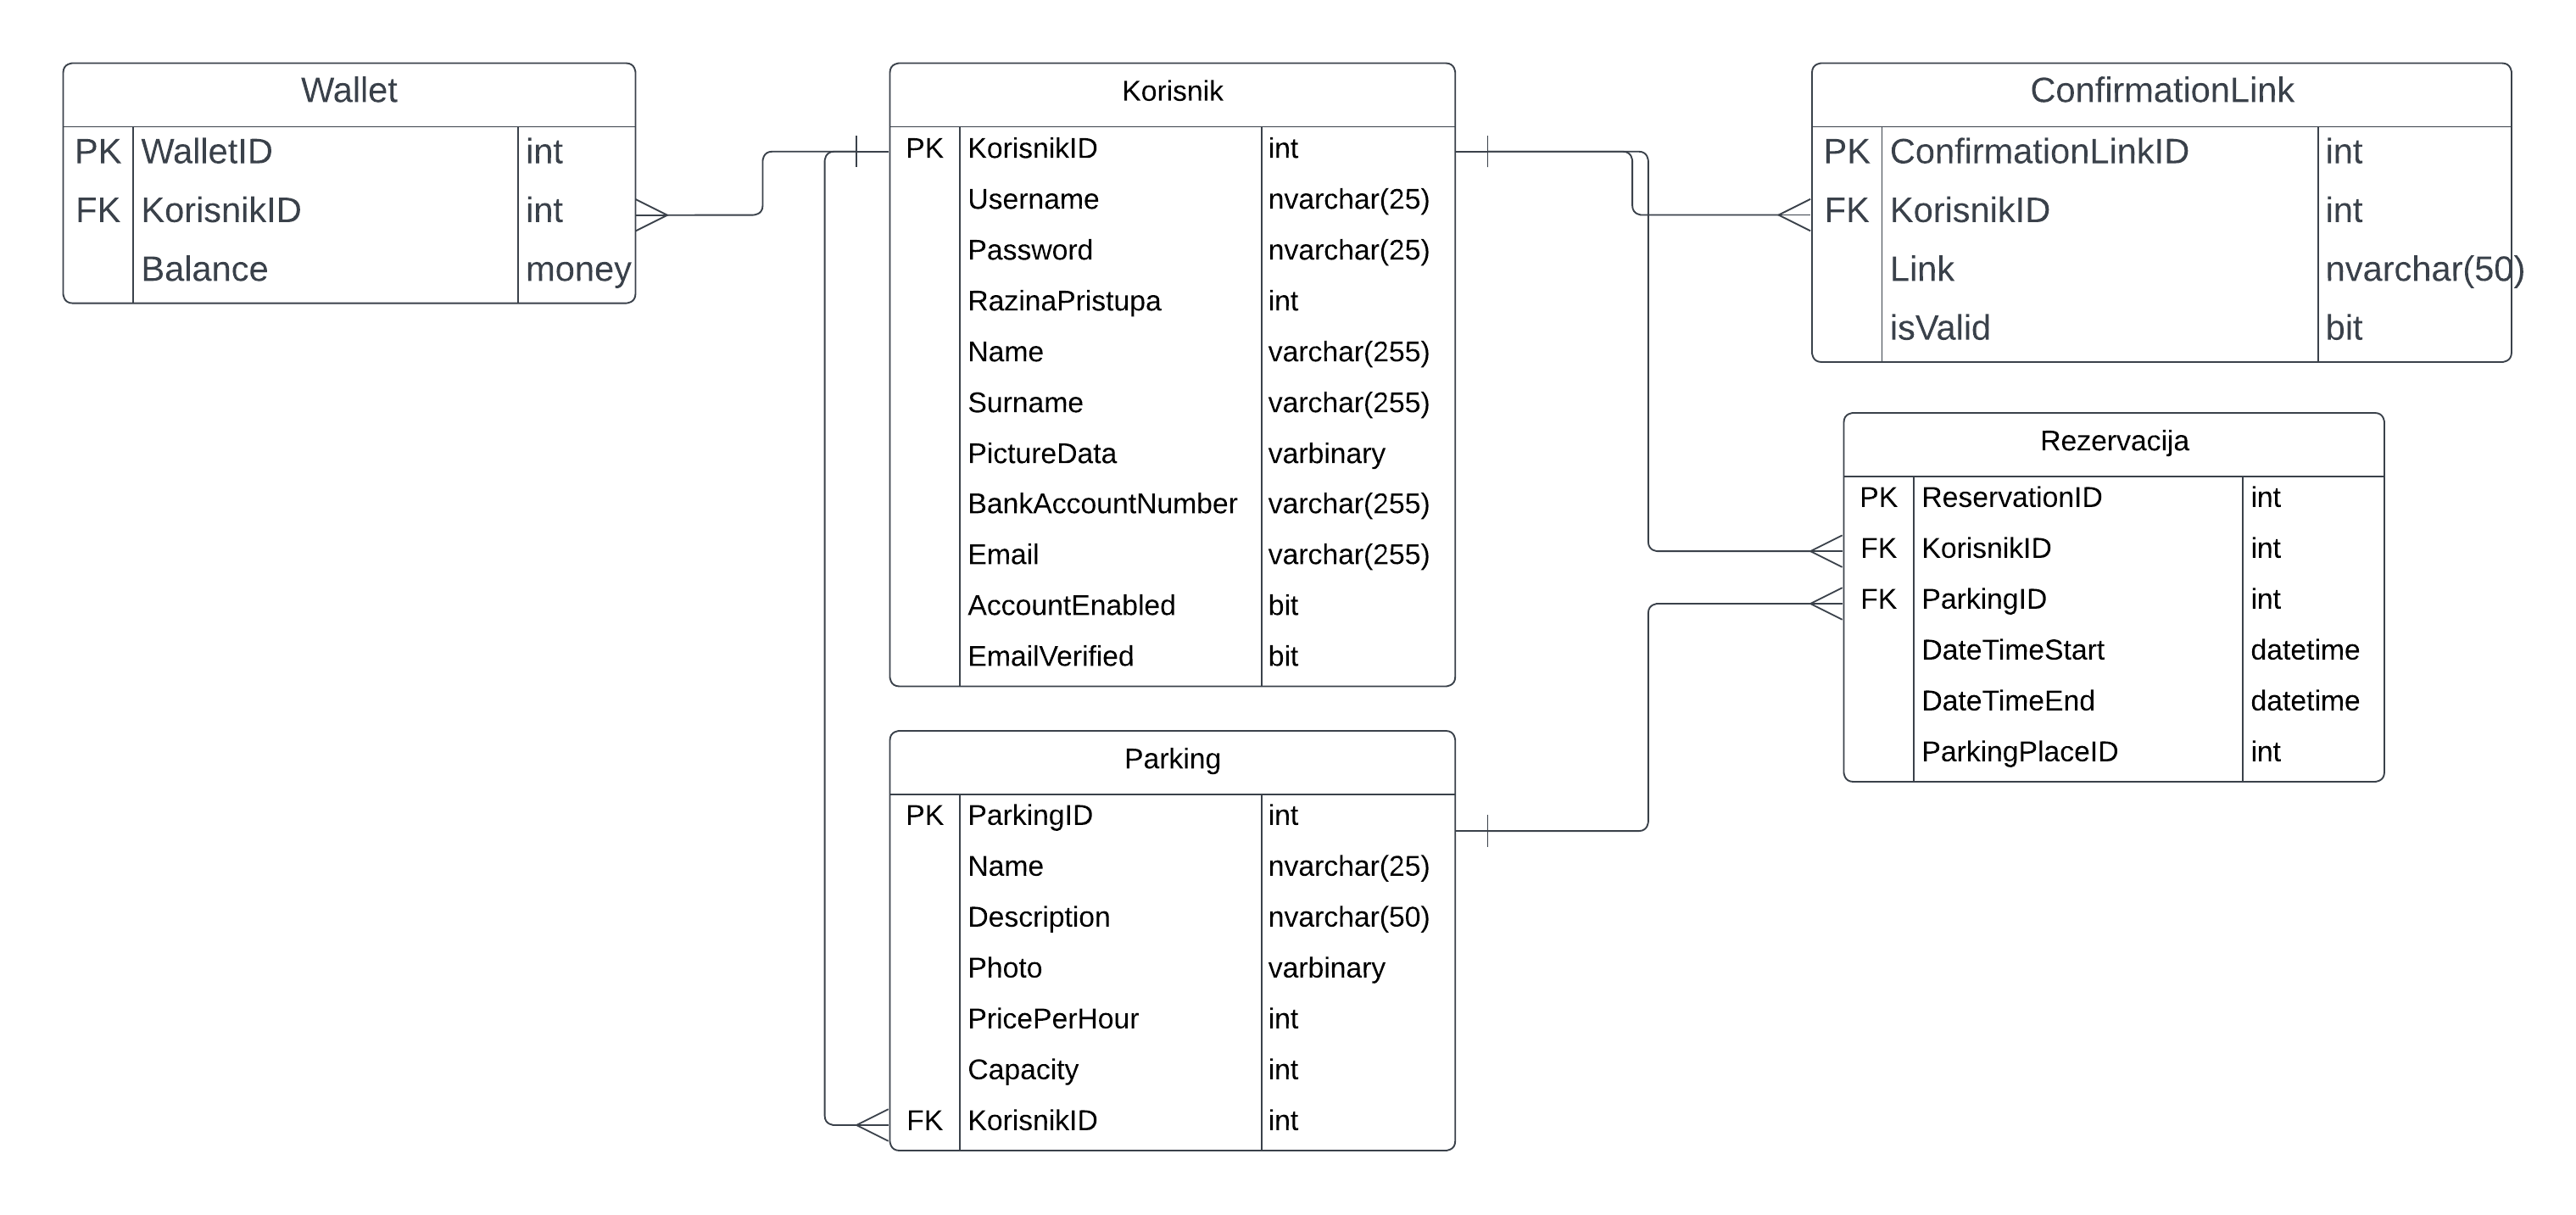
\includegraphics[width=1\linewidth]{dijagrami/ERdijagramPROGI.png}
	\caption{ ER dijagram baze podataka}
	\label{fig:dijagramklijent}
\end{figure}

\section{Dijagram razreda i opis razreda}


\eject